\documentclass[10pt]{article}
\usepackage{icmlko}

\icmlmeta{IP 파운데이션 월드모델}{112}{두 개의 시계}{방향표는 검정을 통과해 그대로 두고, 시간 분할의 두 규약을 코드에 박았다 --- 판정치는 두 규약 모두 네 시점 전부 양수다}

\begin{document}

\twocolumn[
\icmlheader

\begin{abstract}
노트 111이 둘을 남겼다. \textbf{① 방향표를 판정한다.} 노트 105 · 108이 자료를
보고 정한 일곱 항목은 채택 절차를 안 거쳤고, 노트 111이 그중 하나(애니의 미디어
홍보)를 되돌리면 판정치가 \emph{오른다}($+$0.0030)는 것을 봤다. 의심스러운 둘을
씨앗 넷 짝지은 붓스트랩에 걸었다. \textbf{전부 보류 12/12다} --- 애니의 미디어
홍보 $+$0.0030(구간 $-$0.0098$\sim+$0.0073), 웹툰의 입장료 $-$0.0002, 둘 다 빼기
$+$0.0039. \textbf{뺄 근거가 없다. 방향표를 그대로 둔다} --- 노트 111의 관측은
점추정이었을 뿐이다. \textbf{② 규약을 코드에 박았다.} 노트 106--111에서 네
노트에 걸쳐 같은 혼동이 났다 --- 시간 분할의 팝업이 음수라 ``안 따라온다''고
적었는데 그 손해의 91\%가 방향표를 다시 정하는 데서 왔다. \texttt{state/twoproto.py}
를 만들어 \textbf{엄격}(방향도 $T$ 이전으로)과 \textbf{배포}(방향표 고정)를
늘 같이 내게 했다. 결과가 분명하다 --- \textbf{판정치는 두 규약 모두 네 시점
전부 양수}이고(엄격 $+$0.0202 · 배포 $+$0.0241), \textbf{갈리는 것은 팝업
하나}다(엄격 $-$0.0352 · 배포 $-$0.0033). 노트 108의 채택이 미래 규약
\emph{둘 다}에서 확인된 셈이다. 하나만 봤다면 또 헷갈렸을 것이다.
\end{abstract}
]

\begin{figure*}[t]
\centering
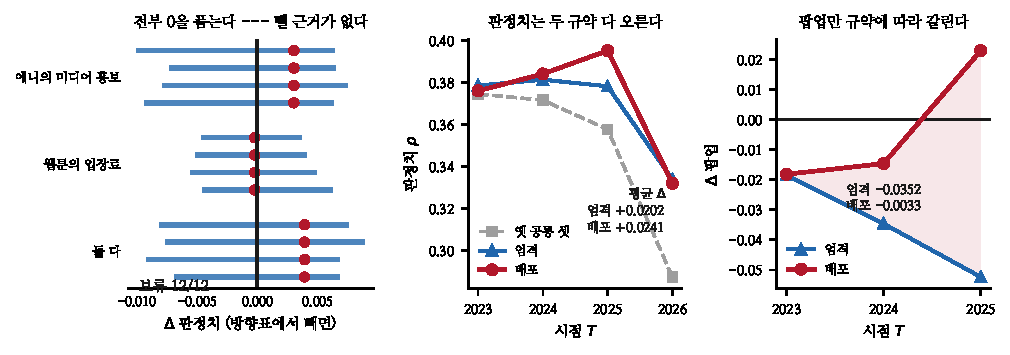
\includegraphics[width=\textwidth]{figs/tc.pdf}
\caption{왼쪽 --- 전부 0을 품는다. 가운데 --- 판정치는 두 규약 다 오른다.
오른쪽 --- 팝업만 규약에 따라 갈린다.}
\end{figure*}

\section{방향표를 판정했다}

방향표는 일곱 항목이다 --- 입장료 여섯 도메인(도서 · 모바일 · 애니 · 웹툰 ·
팝업 · 펀딩)과 미디어 홍보 한 도메인(애니). 노트 111이 하나씩 되돌려 본
결과 다섯은 분명히 필요했고($-$0.003$\sim-$0.019) 둘이 의심스러웠다.

\begin{table}[t]
\centering\tsize
\caption{방향표에서 빼면. 씨앗 넷 · 짝지은 붓스트랩 60회.}
\begin{tabular}{lrl}
\toprule
& $\Delta$판정치 & 95\% 구간 \\
\midrule
애니의 미디어 홍보 & $+$0.0030 & $-$0.0098 $\sim$ $+$0.0073 \\
웹툰의 입장료 & $-$0.0002 & $-$0.0053 $\sim$ $+$0.0061 \\
둘 다 & $+$0.0039 & $-$0.0090 $\sim$ $+$0.0087 \\
\midrule
\multicolumn{3}{l}{\textbf{보류 12/12 --- 방향표를 그대로 둔다}} \\
\bottomrule
\end{tabular}
\end{table}

\claimx{노트 111의 ``애니의 미디어 홍보가 판정치에 해롭다''는 \textbf{점추정이었을
뿐이다.} $+$0.0030 의 구간이 $[-0.0098, +0.0073]$ 로 0을 품고, 팝업은
$-$0.0045로 오히려 나빠진다. \textbf{뺄 근거가 없다.}}{붓스트랩을 60회로
줄였다(보통 100회). 구간이 조금 넓어졌을 수 있는데, 점추정이 구간 한가운데
있어 결론이 바뀔 폭은 아니다.}

\begin{quote}\fontsize{9.5}{11.5}\selectfont
방향표 자체가 이제 채택 절차를 거친 것이 된다. 노트 105 · 108이 자료를 보고
정하고, 노트 111이 하나씩 되돌려 크기를 재고, 이 노트가 의심스러운 것을
검정했다. \textbf{세 단계를 다 밟은 첫 설정}이다.
\end{quote}

\section{규약을 코드에 박았다}

노트 106--111에서 네 노트에 걸쳐 같은 혼동이 났다. 시간 분할의 팝업 수치
하나만 보고 ``팝업이 안 따라온다''를 네 번 적었는데, 노트 111이 그 손해의
91\%가 방향표를 다시 정하는 데서 온다는 것을 보였다. \textbf{둘을 같이 안
보면 되풀이된다.}

\begin{quote}\fontsize{9.0}{11}\selectfont\ttfamily
python3 -m state.twoproto\\[.4em]
\rm 엄격 --- 방향도 $T$ 이전으로 다시 정한다. 못 정하면 그 축을 끈다.\\
\rm\hphantom{엄격 --- }묻는 것: ``그때 이 설계를 내릴 수 있었나''\\[.2em]
\rm 배포 --- 방향표를 고정하고 출처만 자른다.\\
\rm\hphantom{배포 --- }묻는 것: ``지금 이 설계로 미래를 맞히나''
\end{quote}

\begin{table}[t]
\centering\tsize
\caption{두 규약. 옛 공통 셋 대비.}
\begin{tabular}{lrrrr}
\toprule
$T$ & 대상 & 옛 공통 & 엄격 & 배포 \\
\midrule
2023 & 9 & $+$0.3746 & $+$0.3786 & $+$0.3761 \\
2024 & 9 & $+$0.3716 & $+$0.3814 & $+$0.3841 \\
2025 & 8 & $+$0.3577 & $+$0.3782 & $+$0.3953 \\
2026 & 6 & $+$0.2873 & $+$0.3337 & $+$0.3319 \\
\midrule
\multicolumn{3}{l}{평균 $\Delta$} & \textbf{$+$0.0202} & \textbf{$+$0.0241} \\
\bottomrule
\end{tabular}
\end{table}

\claimx{\textbf{판정치는 두 규약 모두 네 시점 전부 양수다}(엄격 $+$0.0202 ·
배포 $+$0.0241). 노트 108의 채택이 미래 규약 \emph{둘 다}에서 확인된다 ---
``그때 내릴 수 있었나''에도 ``지금 맞히나''에도 그렇다.}{시점이 최근일수록
대상 수가 준다(9 $\to$ 6). 시점 \emph{간} 비교는 분모가 다르지만 시점
\emph{안}의 세 수치는 같은 대상 집합에서 나왔다.}

\begin{table}[t]
\centering\tsize
\caption{팝업만 갈린다.}
\begin{tabular}{lrr}
\toprule
$T$ & 엄격 & 배포 \\
\midrule
2023 & $-$0.0185 & $-$0.0182 \\
2024 & $-$0.0347 & $-$0.0146 \\
2025 & $-$0.0524 & \textbf{$+$0.0229} \\
\midrule
평균 & $-$0.0352 & \textbf{$-$0.0033} \\
\bottomrule
\end{tabular}
\end{table}

\claimx{\textbf{갈리는 것은 팝업 하나다.} 판정치는 두 규약이 $+$0.0202와
$+$0.0241로 거의 같은데 팝업은 $-$0.0352와 $-$0.0033으로 열 배 넘게 다르다.
팝업만 과거가 없기 때문이며(노트 111), 그래서 \textbf{팝업 수치는 규약을
밝히지 않으면 읽을 수 없다.}}{배포 규약이 낙관적이다. 방향표가 전체 자료에서
나왔으므로 미래 평가에 그만큼 누출이 있다.}

\section{앞으로의 규약}

\begin{table}[t]
\centering\tsize
\caption{어느 수치를 어디에 쓰나.}
\begin{tabular}{ll}
\toprule
설계 결정(축 · 배선 · 성분) & 판정치 --- 씨앗 넷 붓스트랩 \\
설계가 미래에도 서나 & \textbf{엄격} 시간 분할 \\
제품이 미래를 맞히나 & \textbf{배포} 시간 분할, 팝업 \\
도메인 집합 결정 & \textbf{아무것도 안 쓴다}(노트 82) \\
제품용 별도 설정 & \textbf{안 둔다}(노트 107) \\
\bottomrule
\end{tabular}
\end{table}

\section{한계}

\begin{itemize}[leftmargin=1.1em,itemsep=0.15em]
\item 방향표 일곱 중 둘만 검정했다. 나머지 다섯은 점추정만 보고 필요하다고
      판단했다($-$0.003$\sim-$0.019).
\item 붓스트랩을 60회로 줄였다.
\item 배포 규약의 방향표 누출을 정량화 못 했다. 노트 105가 보정 50\%로 같은
      표가 나옴을 보였을 뿐이다.
\item 만화 · 세계애니가 왜 팝업 전이를 깎는지 여전히 모른다(노트 111).
\item $T{=}2026$ 은 팝업 이후 레코드가 19건이라 팝업 수치가 없다.
\end{itemize}

\section{다음}

\begin{enumerate}[leftmargin=1.3em,itemsep=0.15em]
\item \textbf{만화 · 세계애니가 왜 깎나} --- 노트 111이 남긴 유일한 미해결.
      두 도메인의 새 축 적재가 팝업의 것과 어떻게 다른지 본다.
\item \textbf{팝업 레코드} --- 노트 92 · 106 · 107 · 110 · 111 · 112가 전부
      같은 곳을 가리킨다. 25건이면 방향을 정하고 510건이면 설계를 판정한다.
      \textbf{모으는 절차를 설계한다.}
\item 방향표 나머지 다섯도 검정한다.
\item 텀블벅 API --- 펀딩만 미디어 홍보 0\%로 남았다.
\end{enumerate}

\vspace{0.6em}
\hrule height 0.3pt
\vspace{0.5em}
{\footnotesize
\textbf{참고문헌}\\[0.3em]
Bergmeir, C., Benitez, J. M. (2012). On the use of cross-validation for time
series predictor evaluation. \emph{Information Sciences}, 191, 192--213.\\[0.15em]
Cawley, G. C., Talbot, N. L. C. (2010). On over-fitting in model selection and
subsequent selection bias in performance evaluation. \emph{JMLR}, 11, 2079--2107.\\[0.15em]
Efron, B., Tibshirani, R. J. (1993). \emph{An Introduction to the Bootstrap}.
Chapman \& Hall.\\[0.15em]
Meredith, W. (1993). Measurement invariance, factor analysis and factorial
invariance. \emph{Psychometrika}, 58(4), 525--543.\\[0.15em]
Ben-David, S. et al. (2010). A theory of learning from different domains.
\emph{Machine Learning}, 79(1--2), 151--175.
}

\end{document}
